\documentclass[12pt, a4paper]{article}

\usepackage[margin=2.5cm]{geometry}
\usepackage{graphicx}
\usepackage{booktabs}
\usepackage{hyperref}
\usepackage{amsmath}
\usepackage{float}
\usepackage{caption}
\usepackage{subcaption}
\usepackage{listings}
\usepackage{xcolor}
\usepackage{parskip}

% Code listing style
\lstset{
    language=Python,
    basicstyle=\ttfamily\small,
    keywordstyle=\color{blue},
    commentstyle=\color{gray},
    stringstyle=\color{purple},
    breaklines=true,
    frame=single,
    numbers=left,
    numberstyle=\tiny\color{gray},
    showstringspaces=false,
    tabsize=4,
}

\hypersetup{colorlinks=false, hidelinks}

% -----------------------------------------------------------------------
\title{
    \vspace{-2cm}
    \textbf{Identification and Classification of Cross-outs in Handwritten Documents} \\
    \large D7047E -- Advanced Deep Learning \\
    \large Project Report
}

\author{} % Custom table used in document body
\date{}   % Custom table used in document body

\begin{document}

\maketitle

\begin{center}
    \vspace{-1cm}
    \textbf{Group 14} \\
    \textit{17 May 2026} \\
    \vspace{0.5cm}
    
    \begin{tabular}{l}
    \toprule
    \textbf{Team Members} \\ \midrule
    Suresh Balaraman \\
    Nagarajan Ganesan \\
    Chirag Gurumurthy \\
    Shameena Mohammed Nabeel \\
    Lakshmi Shankar Paramasivan \\ \bottomrule
    \end{tabular}
\end{center}

\tableofcontents
\newpage

% -----------------------------------------------------------------------
\section{Abstract}
Handwritten text recognition (HTR) is a critical task in document analysis, yet it is often hindered by the presence of cross-outs, where words are marked with lines or scribbles. These artifacts obscure content and significantly affect recognition accuracy. This project develops a deep learning-based approach to automatically identify and classify seven types of synthetic cross-outs applied to the IAM dataset. We propose a multi-stage pipeline involving binary detection and multi-class classification. Furthermore, we evaluate model robustness through a custom-curated dataset of 56 images to ensure generalization across unseen handwriting styles.

% -----------------------------------------------------------------------
\section{Introduction}

Cross-outs in handwritten documents signify author edits but act as noise for automated recognition systems \cite{handout}. This project develops a deep learning pipeline to (1) detect crossed-out words (binary), (2) classify the cross-out style into one of seven types, and (3) evaluate generalisation on a custom dataset of 56 real hand-drawn images \cite{handout}.

% -----------------------------------------------------------------------
\section{Background and Model Selection}
\label{sec:lit_review}

Deep learning has become the dominant approach for artifact classification in handwritten documents:
\begin{itemize}
    \item \textbf{CNNs} (ResNet, EfficientNet): learn hierarchical spatial features effective for local stroke patterns.
    \item \textbf{Transfer Learning:} fine-tuning ImageNet pre-trained models achieves high accuracy with limited document data.
    \item \textbf{Vision Transformers (ViT):} capture long-range spatial dependencies via self-attention — useful for patterns like diagonal or zig-zag cross-outs spanning entire words.
\end{itemize}

% -----------------------------------------------------------------------
\section{Method}
\label{sec:method}

\subsection{Dataset and Structure}

The project uses a modified IAM Handwriting Database \cite{iam_db} with seven synthetic cross-out styles: Single-Line, Double-Line, Diagonal, Cross, Wave, Zig-zag, and Scratch — plus a \texttt{CLEAN} and \texttt{MIXED} class. For binary classification all styles and \texttt{MIXED} collapse into one positive class (1:8 imbalance); for multi-class, \texttt{MIXED} is excluded leaving eight balanced classes (Table~\ref{tab:dataset_splits}).

\begin{table}[H]
\centering
\caption{Dataset Splits}
\label{tab:dataset_splits}
\begin{tabular}{lrrr}
\toprule
\textbf{Split} & \textbf{CLEAN} & \textbf{CROSSED$^\dagger$} & \textbf{MC per class$^\ddagger$} \\ \midrule
Train & 47{,}997 & 383{,}976 & 47{,}997 \\
Val   & 7{,}559  & 60{,}472  & 7{,}559  \\
Test  & 20{,}306 & 162{,}448 & 20{,}306 \\ \bottomrule
\multicolumn{4}{l}{\footnotesize $^\dagger$ 7 styles + MIXED (8 $\times$ 47,997 per split).} \\
\multicolumn{4}{l}{\footnotesize $^\ddagger$ Multi-class: 8 balanced classes (MIXED excluded).}
\end{tabular}
\end{table}

\subsection{Preprocessing Pipeline and Data Augmentation}
\label{sec:preproc}

\begin{table}[H]
\centering
\caption{Preprocessing and Augmentation Pipeline}
\label{tab:preproc}
\begin{tabular}{lll}
\toprule
\textbf{Transform} & \textbf{Parameters} & \textbf{Purpose} \\ \midrule
\multicolumn{3}{l}{\textit{Deterministic (train, val, test)}} \\
Grayscale $\to$ 3-channel & — & ImageNet compatibility \\
PadToSquare & fill=255 & Preserve stroke aspect ratio \\
Resize & $224\times224$ & Architecture input requirement \\
Normalize & ImageNet $\mu$/$\sigma$ & Consistent with pre-trained weights \\ \midrule
\multicolumn{3}{l}{\textit{Stochastic (training only)}} \\
RandomRotation & $\pm5^\circ$ & Tilted paper/camera \\
RandomAffine & 5\% translation & Positional shift robustness \\
RandomPerspective & distortion 0.2, $p{=}0.5$ & Angled photo capture \\
GaussianBlur & $\sigma\in[0.1,1.0]$ & Camera blur / low-res scanning \\
ColorJitter & brightness \& contrast $\pm0.3$ & Variable lighting \\ \bottomrule
\end{tabular}
\end{table}

\subsection{Implementation Strategy}

A two-stage pipeline was implemented: Stage 1 (binary) detects whether a word is crossed out; Stage 2 (multiclass) identifies the style. SimpleCNN (trained from scratch) is the final model for both tasks. ResNet-50 and ViT-B/16 were explored as alternatives. Generalisation is assessed on a custom dataset of 56 real hand-drawn images.

% -----------------------------------------------------------------------
\subsection{Binary Classification}
\label{sec:binary}

\subsubsection{Task Definition}

CLEAN (label 0) vs.\ CROSSED-OUT (label 1); all seven styles and \texttt{MIXED} collapsed into the positive class. The 1:8 class imbalance (Table~\ref{tab:dataset_splits}) is addressed with class-weighted cross-entropy.

\subsubsection{Architecture}

The selected model is \textbf{SimpleCNN}, a custom CNN trained from scratch with 7 convolutional layers organised into four blocks, all using $3{\times}3$ kernels with BatchNorm and ReLU:

\begin{itemize}
    \item Block 1 ($224{\to}112$): Conv(3${\to}$32) $\times$2 + MaxPool
    \item Block 2 ($112{\to}56$): Conv(32${\to}$64) $\times$2 + MaxPool
    \item Block 3 ($56{\times}56$, no pool): Conv(64${\to}$128) + Conv(128${\to}$128) — preserves spatial detail
    \item Block 4 ($56{\times}56$, no pool): Conv(128${\to}$256) + AdaptiveAvgPool($7{\times}7$)
\end{itemize}

Classifier head: $\text{Flatten}(12{,}544) \to \text{Linear}(512) \to \text{ReLU} \to \text{Dropout}(0.4) \to \text{Linear}(128) \to \text{ReLU} \to \text{Dropout}(0.3) \to \text{Linear}(2)$. Total trainable parameters: 7.07M.

We also conducted early-epoch trials with ResNet-50 and ViT-B/16 (ImageNet pre-trained, frozen backbone). After observing that SimpleCNN matched or exceeded their validation accuracy within the first 5--10 epochs while being significantly faster to train, we proceeded exclusively with SimpleCNN for the binary task.

\subsubsection{Training Configuration}

Table~\ref{tab:hparams} summarises the hyperparameters for all models across both tasks.

\begin{table}[H]
\centering
\caption{Training Hyperparameters --- All Models}
\label{tab:hparams}
\begin{tabular}{llll}
\toprule
\textbf{Hyperparameter} & \textbf{Binary (SimpleCNN)} & \textbf{MC (SimpleCNN)} & \textbf{MC (ResNet-50)} \\ \midrule
Optimizer               & Adam          & Adam         & Adam \\
Learning rate           & $10^{-3}$     & $10^{-4}$    & $4\times10^{-4}$ \\
LR scheduler            & \multicolumn{3}{c}{ReduceLROnPlateau (factor=0.1, patience=5, min\_lr=$10^{-6}$)} \\
Batch size              & 64            & 64           & 256 \\
Max / Min epochs        & \multicolumn{3}{c}{100 / 20} \\
Early stopping          & \multicolumn{3}{c}{15 epochs} \\
Loss function           & Wtd.\ CE (1:8) & \multicolumn{2}{c}{Cross-Entropy (balanced classes)} \\
Unfrozen layers         & All           & All          & layer4 + fc head \\ \bottomrule
\end{tabular}
\end{table}

\paragraph{Regularization.}
Dropout ($p{=}0.4$, $p{=}0.3$) and BatchNorm in the classifier head; class-weighted loss (factor 8) for the 1:8 imbalance; ReduceLROnPlateau and early stopping as per Table~\ref{tab:hparams}; data augmentation (Section~\ref{sec:preproc}) as the primary input-space regularizer.

\subsubsection{Results}

Table~\ref{tab:binary_results} summarises performance on the IAM test set and the custom evaluation set.

\begin{table}[H]
\centering
\caption{Binary Classification --- SimpleCNN Results}
\label{tab:binary_results}
\begin{tabular}{lcc}
\toprule
\textbf{Metric} & \textbf{IAM Test Set} & \textbf{Custom Dataset} \\ \midrule
F1 Score           & 0.9908 & 0.9320 \\
Generalisation Gap & \multicolumn{2}{c}{0.0587} \\ \bottomrule
\end{tabular}
\end{table}

\begin{figure}[htbp]
\centering
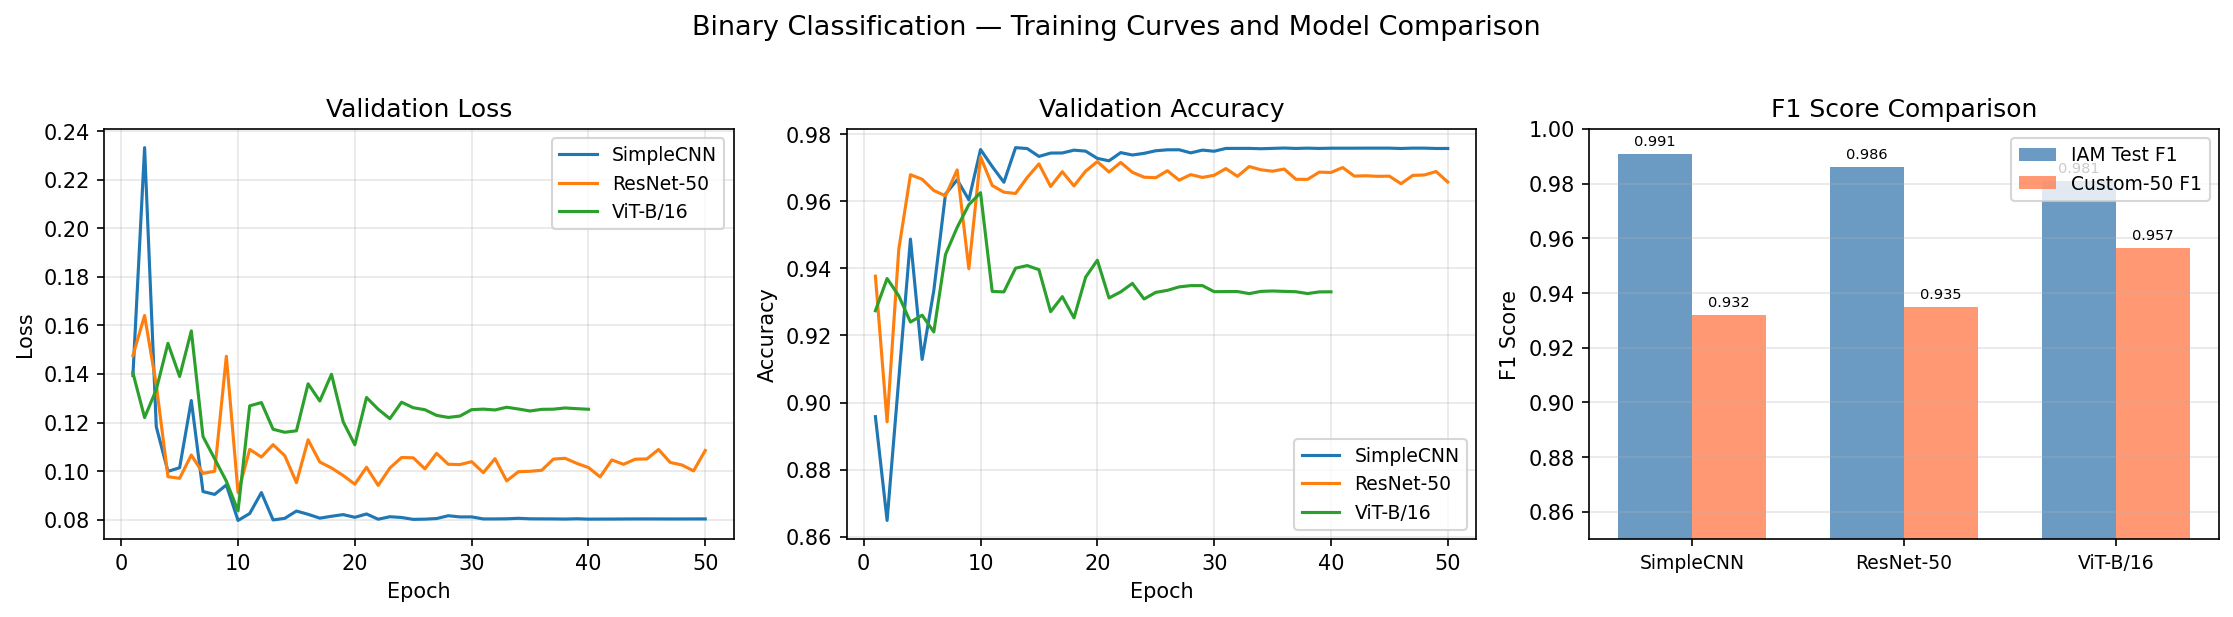
\includegraphics[width=0.75\textwidth]{wandb/binary/binary_training_curves.png}
\caption{Binary classification training curves: SimpleCNN, ResNet-50, and ViT-B/16.}
\label{fig:binary_curves}
\end{figure}

SimpleCNN achieved IAM F1 = 0.991, converging within $\sim$5 epochs, and generalises well to the custom evaluation set (F1 = 0.932, gap = 0.059). ResNet-50 and ViT-B/16 were trialled but discontinued after 5--10 epochs as SimpleCNN matched their validation accuracy at significantly lower training cost.

% -----------------------------------------------------------------------
\subsection{Multi-class Classification}
\label{sec:multiclass}

\subsubsection{Task Definition}

Eight balanced classes: \texttt{CLEAN} plus the seven cross-out styles. \texttt{MIXED} is excluded as it has no specific style label (see Table~\ref{tab:dataset_splits}).

\subsubsection{Architectures}

Two architectures were trained and compared:

\paragraph{SimpleCNN.} The same architecture described in Section~\ref{sec:binary}, with the output layer widened to 8 classes. Trained from scratch with LR $= 10^{-4}$, batch size 64.

\paragraph{ResNet-50.} Pre-trained on ImageNet. Unlike the binary variant where the entire backbone was frozen, here \textbf{layer4} (the final residual block, $\sim$8.4M parameters) is unfrozen alongside the classification head to allow fine-grained feature adaptation. The head is: $\text{Linear}(2048 \to 512) \to \text{ReLU} \to \text{Dropout}(0.3) \to \text{Linear}(512 \to 8)$. Trained with LR $= 4 \times 10^{-4}$, batch size 256.

\subsubsection{Training Configuration}

Hyperparameters follow Table~\ref{tab:hparams}. Both models use the same ReduceLROnPlateau scheduler, early stopping, and epoch budget; they differ in learning rate, batch size, and unfrozen layers.

\subsubsection{Results}

\paragraph{IAM Test Set.}
Table~\ref{tab:mc_results} summarises IAM test set performance for both models.

\begin{table}[H]
\centering
\caption{Multi-class Classification --- IAM Test Set Results}
\label{tab:mc_results}
\begin{tabular}{lcccc}
\toprule
\textbf{Model} & \textbf{Val Acc} & \textbf{Test Acc} & \textbf{Macro-F1} & \textbf{Custom Dataset F1} \\ \midrule
ResNet-50  & 0.8947 & 0.9025 & 0.9098 & --- \\
SimpleCNN  & 0.8957 & 0.9042 & 0.9130 & 0.485 \\ \bottomrule
\end{tabular}
\end{table}

\paragraph{Training dynamics.}
Both models converged to $\approx$0.895 validation accuracy (ResNet-50 in 55 epochs, SimpleCNN in 77). Despite training longer, SimpleCNN achieved marginally higher test accuracy (0.9042 vs.\ 0.9025) and Macro-F1 (0.9130 vs.\ 0.9098).

\begin{figure}[htbp]
\centering
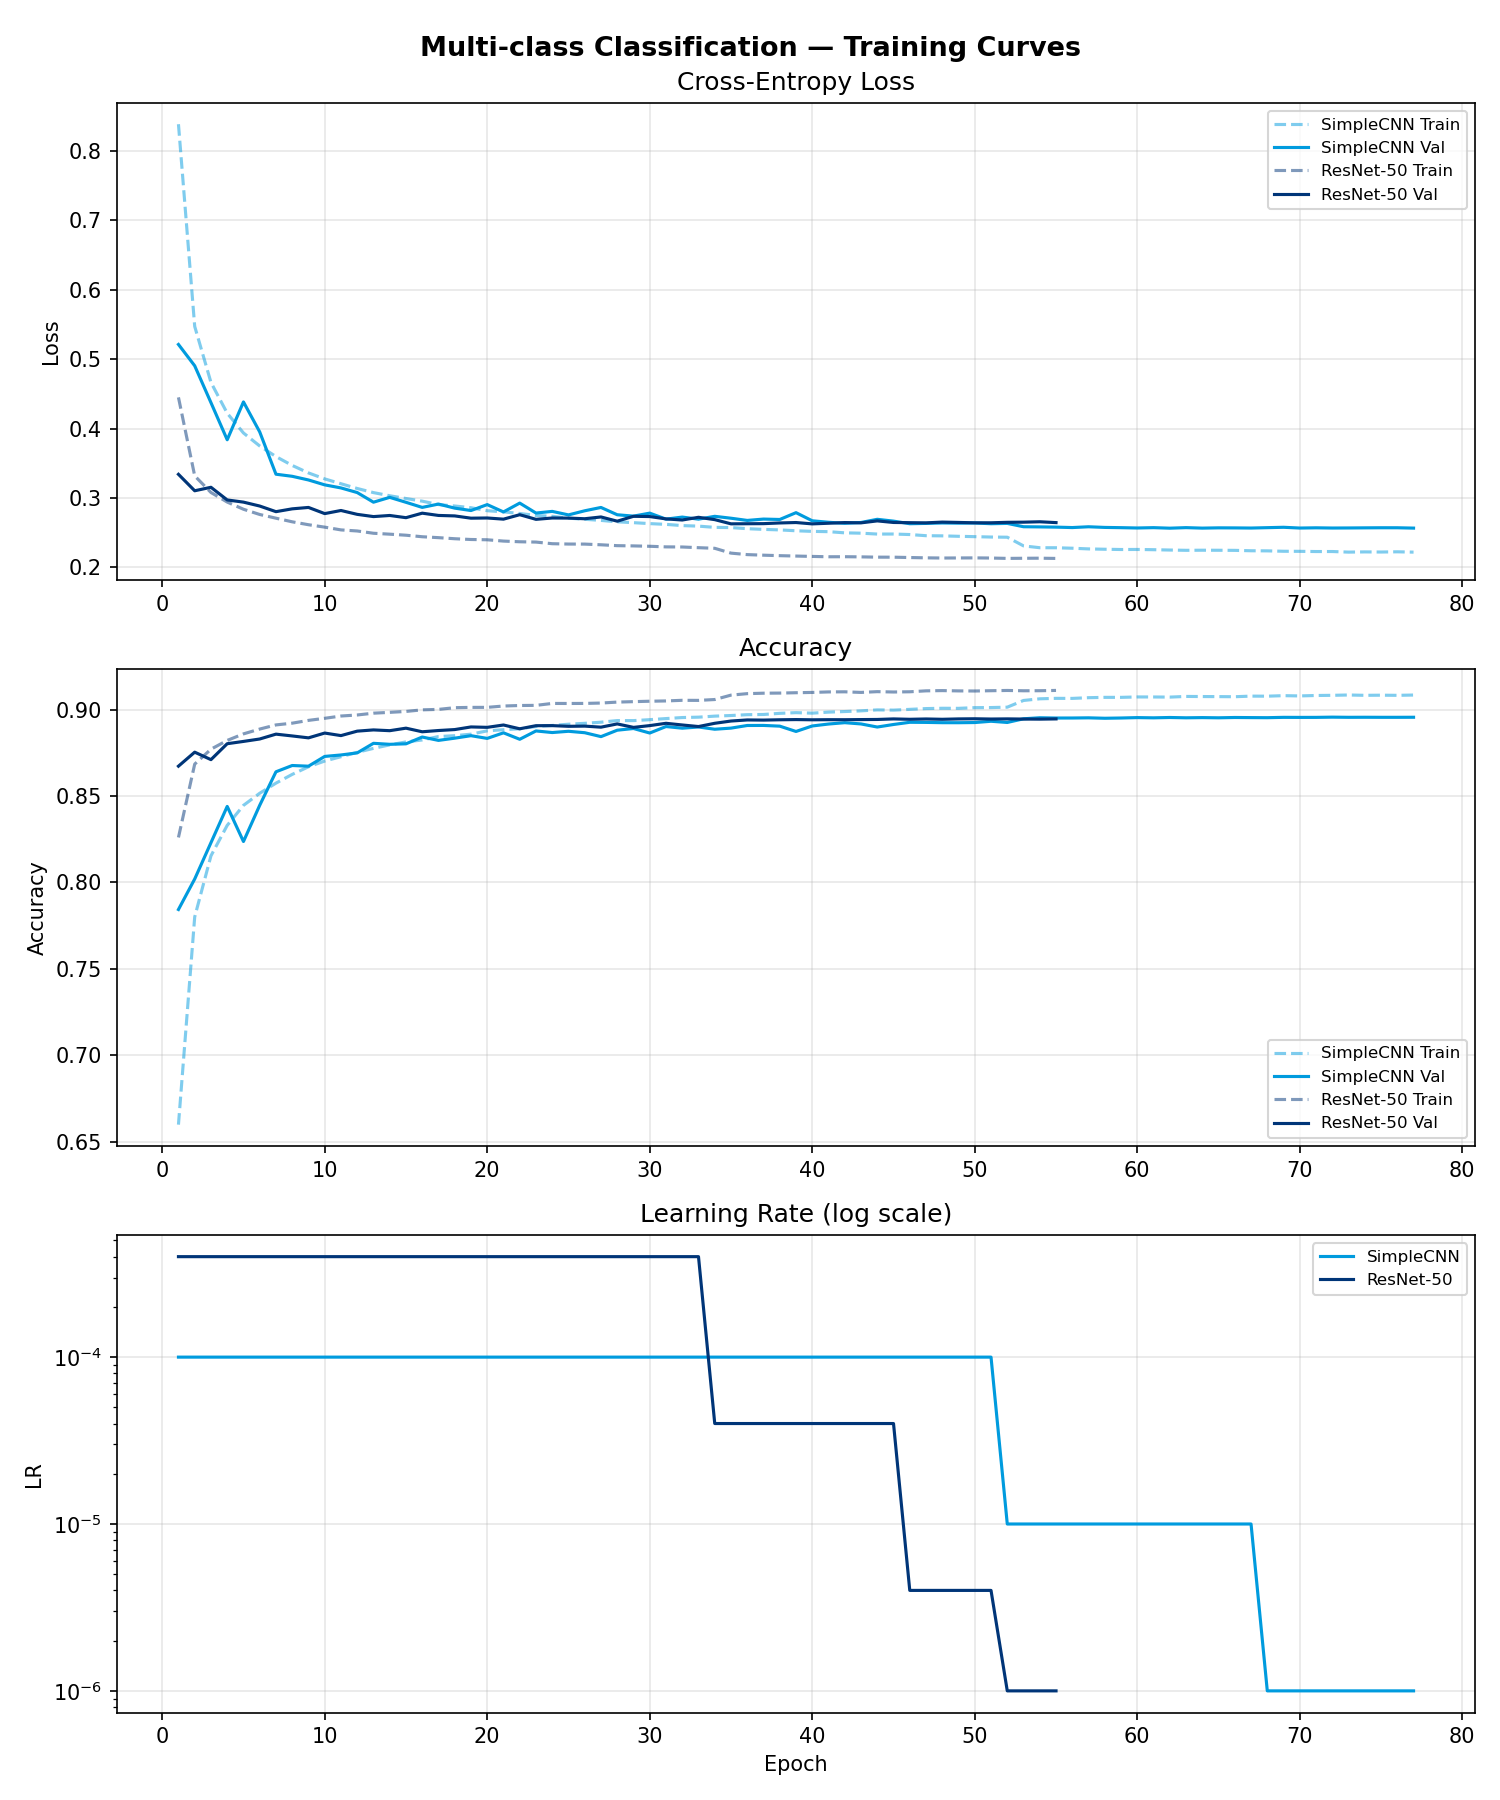
\includegraphics[width=0.75\textwidth]{wandb/multiclass/mc_training_curves.png}
\caption{Multi-class training curves: ResNet-50 vs.\ SimpleCNN.}
\label{fig:mc_curves}
\end{figure}

\paragraph{Confusion matrix analysis.}
Both models show systematic \textbf{ZIG\_ZAG over-prediction} ($\approx$9--10\% of every class), with WAVE most affected in ResNet-50 (12.9\%). SimpleCNN's pattern is slightly attenuated, consistent with its higher Macro-F1 (Figure~\ref{fig:mc_cm}).

\begin{figure}[H]
\centering
\begin{subfigure}[b]{0.44\textwidth}
    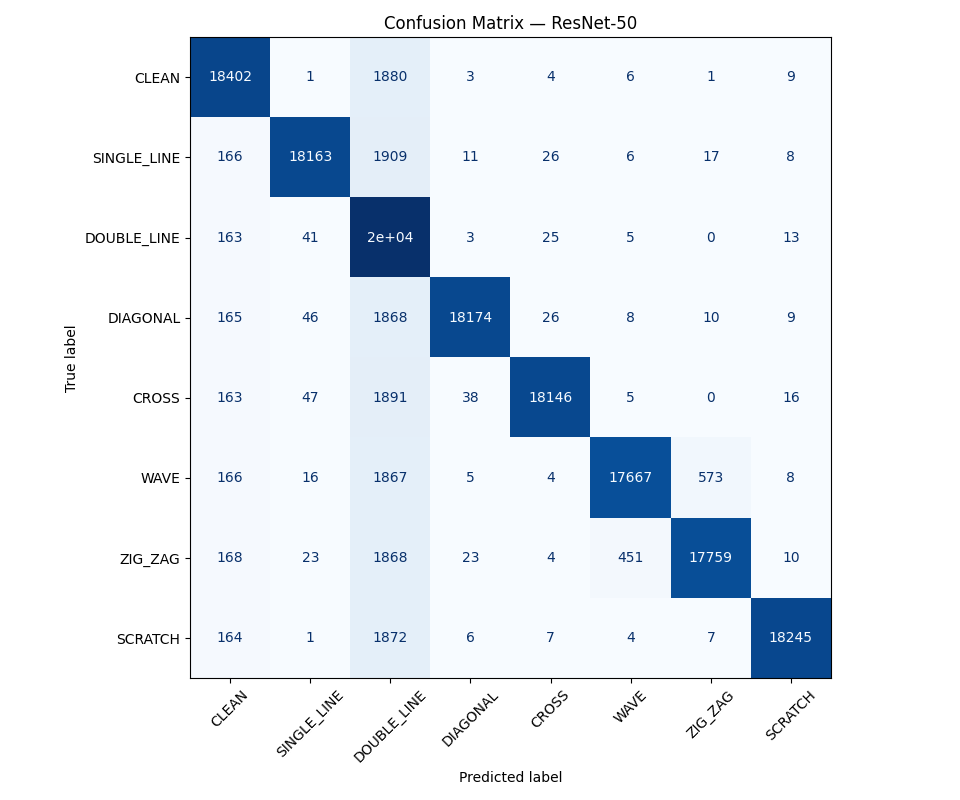
\includegraphics[width=\textwidth]{wandb/multiclass/resnet_confusion_matrix.png}
    \caption{ResNet-50}
    \label{fig:mc_cm_resnet}
\end{subfigure}
\hfill
\begin{subfigure}[b]{0.44\textwidth}
    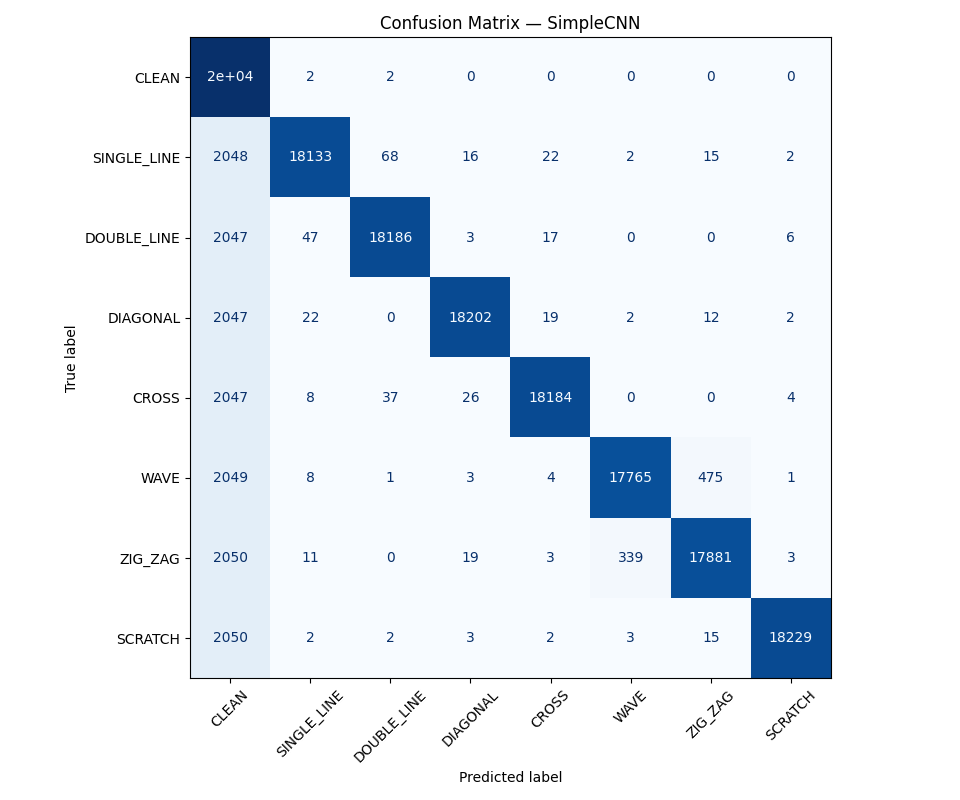
\includegraphics[width=\textwidth]{wandb/multiclass/simplecnn_confusion_matrix.png}
    \caption{SimpleCNN}
    \label{fig:mc_cm_simplecnn}
\end{subfigure}
\caption{Confusion matrices on the IAM test set. SGL = Single-Line, DBL = Double-Line, DIAG = Diagonal, ZZ = Zig-Zag.}
\label{fig:mc_cm}
\end{figure}

\paragraph{Model selection.}
\textbf{SimpleCNN} is selected as the final multiclass model:
\begin{itemize}
    \item Higher Macro-F1 (0.9130 vs.\ 0.9098) and test accuracy (0.9042 vs.\ 0.9025)
    \item Lighter: 7.07M vs.\ $\sim$25M parameters
    \item ResNet-50's DOUBLE\_LINE over-prediction is an ImageNet pretraining artifact requiring costly deeper unfreezing
    \item Consistent with the binary task choice
\end{itemize}

\paragraph{Custom Dataset Generalisation.}
SimpleCNN drops to Macro-F1 = 0.485 (gap = 0.428 vs.\ IAM), per Table~\ref{tab:mc_custom50} and Figure~\ref{fig:mc_cm_custom50}. Three failure modes emerge:
\begin{itemize}
    \item \textbf{WAVE \& ZIG\_ZAG → CLEAN}: real strokes are lighter and less uniform than synthetic training examples.
    \item \textbf{SINGLE\_LINE, DOUBLE\_LINE \& CROSS → DIAGONAL}: natural hand-drawn lines carry a slight angle vs.\ perfectly horizontal synthetic strokes.
    \item \textbf{CLEAN \& SCRATCH robust} (F1 = 1.0 each): unambiguous appearance survives the domain shift.
\end{itemize}
Root cause: the \textbf{synthetic-to-real domain gap} — clean 300 dpi IAM scans vs.\ hand-photographed images with variable lighting, stroke pressure, and perspective.

\begin{figure}[H]
\centering
\begin{minipage}[c]{0.48\textwidth}
\centering
\captionof{table}{Custom Dataset Per-Class Results (SimpleCNN)}
\label{tab:mc_custom50}
\begin{tabular}{lccc}
\toprule
\textbf{Class} & \textbf{P} & \textbf{R} & \textbf{F1} \\ \midrule
CLEAN        & 0.33 & 1.00 & 0.50 \\
SINGLE\_LINE  & 0.50 & 0.14 & 0.22 \\
DOUBLE\_LINE  & 0.40 & 0.29 & 0.33 \\
DIAGONAL     & 0.55 & 0.86 & 0.67 \\
CROSS        & 0.75 & 0.43 & 0.55 \\
WAVE         & 1.00 & 0.14 & 0.25 \\
ZIG\_ZAG     & 1.00 & 0.29 & 0.44 \\
SCRATCH      & 1.00 & 1.00 & 1.00 \\ \midrule
Macro avg    & 0.69 & 0.52 & 0.49 \\ \bottomrule
\end{tabular}
\end{minipage}
\hfill
\begin{minipage}[c]{0.48\textwidth}
\centering
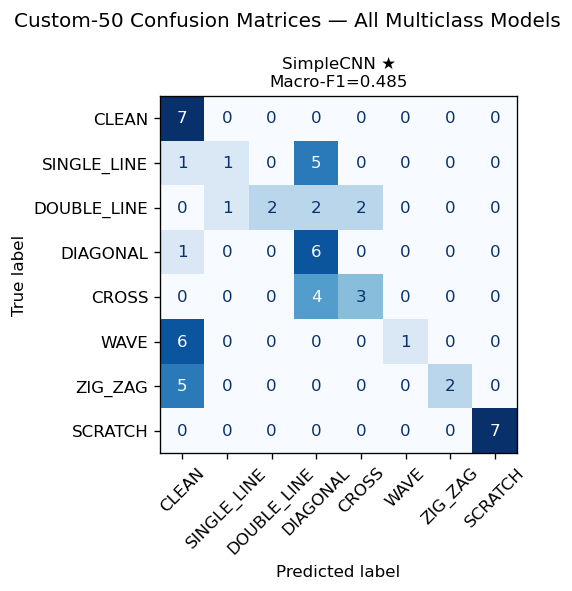
\includegraphics[width=\textwidth]{wandb/custom_eval/custom50_mc_all_cm.png}
\captionof{figure}{Confusion matrix on the custom dataset (Macro-F1 = 0.485).}
\label{fig:mc_cm_custom50}
\end{minipage}
\vspace{0.5em}

\centering
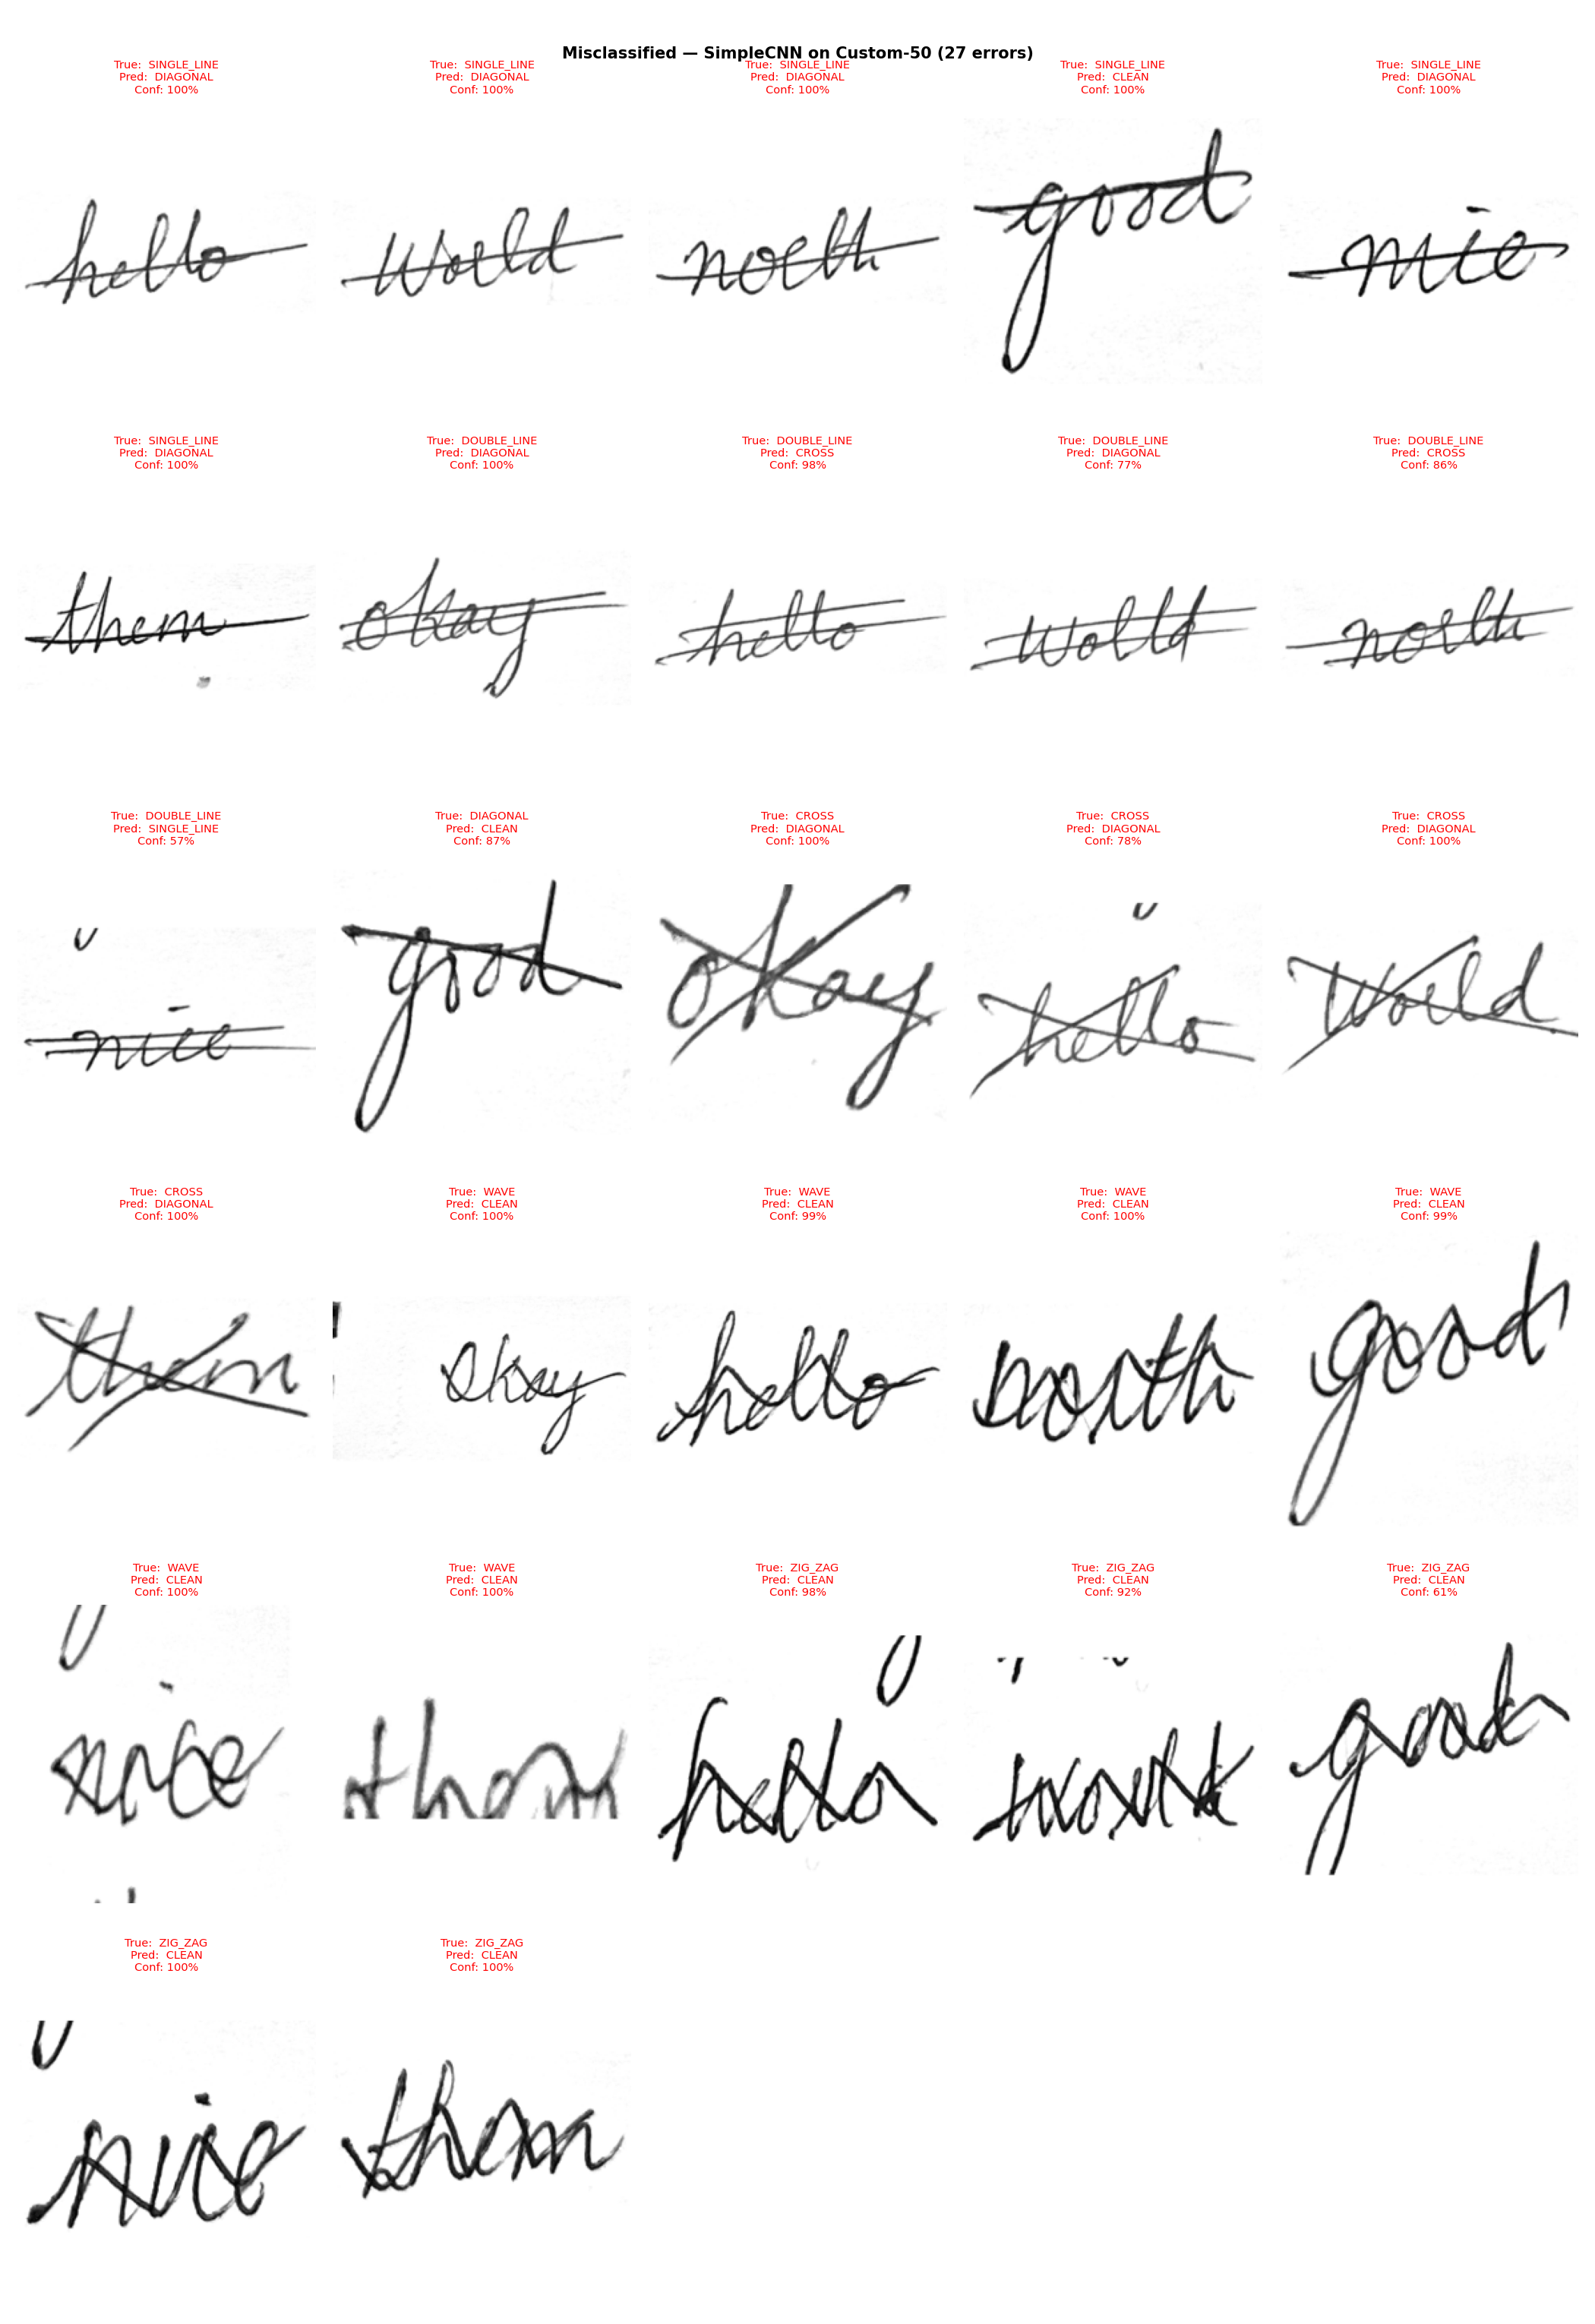
\includegraphics[width=0.65\textwidth]{wandb/custom_eval/custom50_mc_misclassified.png}
\captionof{figure}{All 27 misclassified examples: WAVE/ZIG\_ZAG → CLEAN (faint strokes); SINGLE\_LINE, DOUBLE\_LINE, CROSS → DIAGONAL (natural hand-drawn angle).}
\label{fig:mc_misclassified_custom50}
\end{figure}

% -----------------------------------------------------------------------
\section{Deliverables}
\label{sec:deliverables}

\begin{enumerate}
    \item \textbf{Source Code and Trained Models:} Codebase and model weights on GitHub \cite{repo_link}, including training notebooks and evaluation scripts.
    \item \textbf{Custom Evaluation Dataset:} 56 real hand-drawn images (8 classes $\times$ 7 words), available at \url{https://github.com/chirag-gurumurthy/D7047E_ADL/tree/project/project/dataset/custom_50}.
    \item \textbf{Final Presentation:} 10-minute presentation covering the problem, pipeline, results, and domain shift analysis (\url{https://github.com/chirag-gurumurthy/D7047E_ADL/tree/project/project/docs/ADL_Group14_Presentation.pptx}).
\end{enumerate}

% -----------------------------------------------------------------------
\begin{thebibliography}{9}

\bibitem{handout}
Pathirage, G. and Barney Smith, E. \textit{ADL Project: Document Analysis}.

\bibitem{iam_db}
Marti, U. and Bunke, H. \textit{The IAM-database: an English sentence database for offline handwriting recognition.}

\bibitem{repo_link}
Gurumurthy, C. \textit{D7047E\_ADL Project Repository}. \url{https://github.com/chirag-gurumurthy/D7047E_ADL/tree/project/project}.

\end{thebibliography}

\end{document}
